\subsection{UC 14 - Telegram - Autenticazione}
		
	\begin{figure}[H]
		\centering
		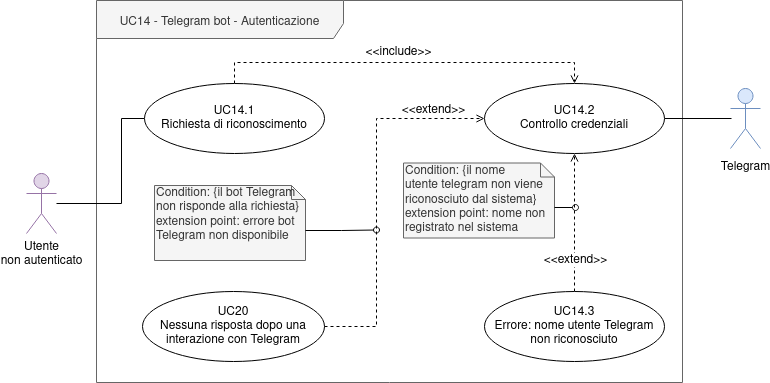
\includegraphics[scale=0.60]{res/images/uc14}
		\caption{Diagramma che descrive il processo di autenticazione tramite Telegram.}
	\end{figure}
		
	\begin{itemize}
		\item \textbf{attori primari:} Utente non autenticato;
		\item \textbf{attori secondari:} \glock{Telegram};
		\item \textbf{descrizione:} l'utente tenta di autenticarsi con il \glock{bot} \glock{Telegram}, per farlo entra all'interno dell'applicazione e inizia la chat con il \glock{bot}. Attraverso \glock{Telegram}, viene segnalato al \glock{bot} il nome utente e il \glock{bot} verifica se questo è censito all'interno del sistema. Se viene riconosciuto, viene registrata l'apertura e l'autenticazione del canale di comunicazione tra il \glock{bot} e l'utente, diventando quest'ultimo autenticato; 
		\item \textbf{precondizione:} l'utente è nell'applicazione di \glock{Telegram} e non ha una chat autenticata con il \glock{bot};
		\item \textbf{postcondizione:} l'utente effettua l'autenticazione e il canale di comunicazione tra utente e \glock{bot} viene salvato nel sistema;
		\item \textbf{scenario principale:}
		\begin{enumerate}
			\item l'utente seleziona nell'applicazione di \glock{Telegram} il \glock{bot} di sistema dal pannello di ricerca;
			\item l'utente tenta di aprire una conversazione con il \glock{bot};
			\item l'utente viene autenticato e la chat viene salvata nel sistema.
		\end{enumerate}
	\end{itemize}
	
	\subsubsection{UC 14.1 - Richiesta di riconoscimento}

	\begin{itemize}
		\item \textbf{attori primari:} Utente non autenticato;
		\item \textbf{descrizione:} l'utente invia una richiesta al \glock{bot} di volersi autenticare per poter aprire il canale di comunicazione;
		\item \textbf{precondizione:} l'utente è nell'applicazione di \glock{Telegram} e non ha una chat autenticata con il \glock{bot};
		\item \textbf{postcondizione:} l'utente invia il comando per richiedere l'autenticazione;
		\item \textbf{scenario principale:}
		\begin{enumerate}
			\item l'utente seleziona nell'applicazione di \glock{Telegram} il \glock{bot} del sistema;
			\item l'utente tenta di aprire una conversazione con il \glock{bot};
			\item per attivare la conversazione con il \glock{bot} ed autenticarsi, l'utente invia il comando predefinito;
		\end{enumerate}
		\item \textbf{inclusioni:}
		\begin{itemize}
			\item Controllo credenziali (UC 14.2).
		\end{itemize}
	\end{itemize}

	\subsubsection{UC 14.2 - Controllo credenziali}

	\begin{itemize}
		\item \textbf{attori primari:} Utente non autenticato;
		\item \textbf{attori secondari:} \glock{Telegram};
		\item \textbf{descrizione:} si deve verificare se il nome utente è stato censito da parte del sistema, così da abilitare la chat di comunicazione ed autenticare l'utente;
		\item \textbf{precondizione:} l'utente, tramite \glock{Telegram}, ha inviato al \glock{bot} una richiesta di avvio conversazione con il comando predefinito;
		\item \textbf{postcondizione:} l'utente effettua il riconoscimento con il sistema e viene autenticato;
		\item \textbf{scenario principale:}
		\begin{enumerate}
			\item il \glock{bot} \glock{Telegram} riceve in input il comando che viene inoltrato al sistema, insieme alle informazioni relative alla chat e all'autore del messaggio;
			\item viene mostrato un messaggio di benvenuto dal \glock{bot}, attraverso \glock{Telegram}, che conferma le credenziali dell'utente;
			\item l'utente viene autenticato e la chat viene salvata nel sistema;
		\end{enumerate}
		\item \textbf{estensioni:}
		\begin{itemize}
			\item Errore: nome utente \glock{Telegram} non riconosciuto (UC 14.3);
			\item Nessuna risposta dopo una interazione con \glock{Telegram} (UC 20).
		\end{itemize}
	\end{itemize}

	\subsubsection{UC 14.3 - Errore: nome utente Telegram non riconosciuto}

	\begin{itemize}
		\item \textbf{attori primari:} Utente non autenticato;
		\item \textbf{descrizione:} l'autenticazione della chat tra il \glock{bot} e l'utente non va a buon fine dal momento che il nome utente associato all'account di \glock{Telegram} non è censito nel sistema;
		\item \textbf{precondizione:} l'utente, tramite \glock{Telegram}, sta tentando di autenticarsi con l'invio del comando predefinito;
		\item \textbf{postcondizione:} l'utente non viene autenticato e viene mostrato un messaggio di errore;
		\item \textbf{scenario principale:}
		\begin{enumerate}
			\item il \glock{bot} \glock{Telegram} riceve in input il comando che viene inoltrato al sistema, insieme alle informazioni relative alla chat e all'autore del messaggio;
			\item viene mostrato un messaggio di errore che segnala che il nome utente associato all'utente \glock{Telegram} non è censito nel sistema;
			\item l'utente non viene autenticato.
		\end{enumerate}
	\end{itemize}